\question{Câu 1}

Thiết kế mạch tổ hợp xấp xỉ phép chia 3.

Để thực hiện phép chia 3, ta có thể sử dụng phương pháp nhân số đó với $\frac{1}{3}$.

Trong đó, ta có thể xấp xỉ $\frac{1}{3}$ $\approx$ $2^{-2}$ + $2^{-4}$ + $2^{-6}$ + $2^{-8}$

Cho các stand cell là: cổng NOT, các LOGIC GATE 2 ngõ vào, MUX 2-1, MUX 4-1.

\answer{a}{Cho ngõ vào là số 32 bit. Thiết kế mạch theo phương pháp đã cho và chỉ sử dụng các standard cell trên.}

Đề bài không yêu cầu thiết kế xấp xỉ phép chia 3 cho số có dấu (bù hai) hoặc số không dấu. Vì vậy, nhóm chọn thiết kế cho số có dấu.

Ý tưởng ban đầu:

- Các phép $\textsf{a}$ $\times$ $2^{-n}$ có thể hiểu là những phép $\textsf{a}$ $>>>$ n (dịch phải có dấu).

- Vì thế $\textsf{a}$ $\times$ $\frac{1}{3}$ $\approx$ ($\textsf{a}$ $>>>$ 2) + ($\textsf{a}$ $>>>$ 4) + ($\textsf{a}$ $>>>$ 6) + ($\textsf{a}$ $>>>$ 8).  

$\Rightarrow$ Thiết kế cần 3 bộ cộng kèm các phép ghép và lặp số để thực hiện.

\vspace{.5cm}

Tối ưu ý tưởng:

- Từ hàm số ban đầu: $2^{-2}$ + $2^{-4}$ + $2^{-6}$ + $2^{-8}$ = $2^{-2}$ + $2^{-4}$ + $2^{-4}$ $\times$ ($2^{-2}$ + $2^{-4}$)

- Vì thế $\textsf{a}$ $\times$ $\frac{1}{3}$ $\approx$ ($\textsf{a}$ $>>>$ 2) + ($\textsf{a}$ $>>>$ 4) + ($\textsf{(($\textsf{a}$ $>>>$ 2) + ($\textsf{a}$ $>>>$ 4))}$ $>>>$ 4)

- Đặt tham số N = ($\textsf{a}$ $>>>$ 2) + ($\textsf{a}$ $>>>$ 4) $\Rightarrow$ $\textsf{a}$ $\times$ $\frac{1}{3}$ $\approx$ N + (N $>>>$ 4)

$\Rightarrow$ Thiết kế cần 2 bộ cộng: 1 để tính toán tham số N và 1 để tính toán N + (N $>>>$ 4).

\vspace{.5cm}

\begin{minipage}[t]{0.5\linewidth}
	$\textsf{*}$ N = ($\textsf{a}$ $>>>$ 4) + ($\textsf{a}$ $>>>$ 2)
	\[
	\renewcommand{\arraystretch}{0.8}
	\begin{array}{@{\hskip1pt}c@{\hskip3pt}c@{\hskip3pt}c@{\hskip3pt}c@{\hskip3pt}c@{\hskip3pt}c@{\hskip3pt}c@{\hskip3pt}c@{\hskip3pt}c@{\hskip3pt}c@{\hskip3pt}c@{\hskip3pt}c@{\hskip1pt}c}
		& a_{31} & a_{31} & a_{31} & a_{31} & a_{31} & a_{30} & \ldots & a_{3} & a_{2} & a_{1} & a_{0} \\[-3pt]
		+ & a_{31} & a_{31} & a_{31} & a_{30} & a_{29} & a_{28} & \ldots & a_{1} & a_{0} \\[-1pt]
		\hline
		& n_{33} & n_{32} & n_{31} & n_{30} & n_{29} & n_{28} & \ldots & n_{3} & n_{2} & n_{1} & n_{0}
	\end{array}
	\]
	
	$\Rightarrow$ Full Adder 34 bit.
\end{minipage}
\begin{minipage}[t]{0.5\linewidth}
	$\textsf{*}$ S = (N $>>>$ 4) + N
	\[
	\renewcommand{\arraystretch}{0.8}
	\begin{array}{@{\hskip1pt}c@{\hskip3pt}c@{\hskip3pt}c@{\hskip3pt}c@{\hskip3pt}c@{\hskip3pt}c@{\hskip3pt}c@{\hskip3pt}c@{\hskip3pt}c@{\hskip3pt}c@{\hskip3pt}c@{\hskip3pt}c@{\hskip3pt}c@{\hskip1pt}c}
		& n_{33} & n_{33} & n_{33} & n_{33} & n_{33} & n_{32} & \ldots & n_{5} & n_{4} & n_{3} & n_{2} & n_{1} & n_{0} \\[-3pt]
		+ & n_{33} & n_{32} & n_{31} & n_{30} & n_{29} & n_{28} & \ldots & n_{1} & n_{0} & & & & \\[-1pt]
		\hline
		& s_{37} & s_{36} & s_{35} & s_{34} & s_{33} & s_{32} & \ldots & s_{5} & s_{4} & s_{3} & s_{2} & s_{1} & s_{0}
	\end{array}
	\]
	
	$\Rightarrow$ Full Adder 36 bit.
\end{minipage}

\vspace{.5cm}

Kết quả ngõ ra Result là 32 bit cao của S.
  

\newpage
\begin{figure}[H]
	\centering
	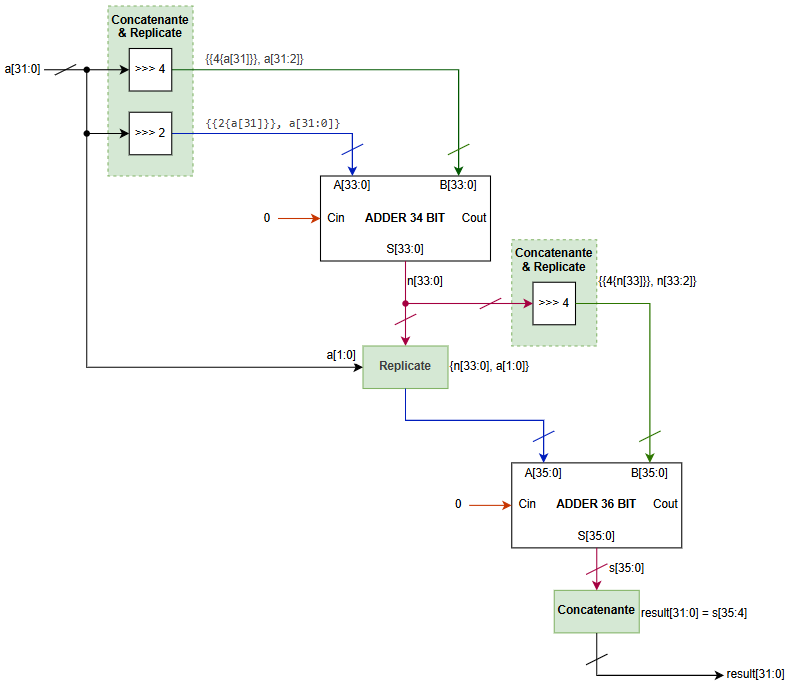
\includegraphics[width=.8\linewidth]{./my-chapters/my-images/Question1/Question1.png}
	\caption{Thiết kế mạch xấp xỉ chia 3.}
\end{figure}

Thiết kế các bộ cộng sẽ được trình bày tại $\textsf{Câu 3}$ và $\textsf{Câu 4}$.

\newpage
\answer{b}{Viết chương trình HDL mô tả mạch đã cho.}
\lstinputlisting[style=StyleCode, language=SystemVerilog, caption={HDL mô tả thiết kế bộ xấp xỉ chia 3.}]{./my-chapters/design_verify/Question1/div_3_estimate.sv}
  

\newpage
\answer{c}{Viết testbench cho mạch, thực hiện testbench với 100 mẫu và tính scoreboard của 100 mẫu đó.}

Nhóm tiến hành kiểm định cho thiết kế bằng phương trình xấp xỉ mà để bài đã cung cấp, vì các hệ số của phương trình là số thực nên nhóm tiến hành tạo ngẫu nhiên 100 giá trị A đầu vào thiết kế là dạng integer. 

Tiến hành ép kiểu A sang dạng shortreal để nhân với ($2^{-2}$ + $2^{-4}$ + $2^{-6}$ + $2^{-8}$).
Sau đó kết quả được ép kiểu lại về dạng integer được sử dụng để so sánh với giá trị đầu ra của thiết kế.

\lstinputlisting[style=StyleCode, language=SystemVerilog, caption={HDL mô tả thiết kế bộ xấp xỉ chia 3.}]{./my-chapters/design_verify/Question1/div_3_tb.sv}

Kết quả:

\begin{lstlisting}[style=StyleResult, language=Result, caption={Kết quả kiểm định cho bộ xấp xỉ chia 3.}]
	xcelium> run
	[TIME:    10] [DIV_3] - FAIL: Expect: 0b0a6d1b, DUT: 0b0a6d13 
	[TIME:    20] [DIV_3] - FAIL: Expect: 24586803, DUT: 245867f1 
	[TIME:    30] [DIV_3] - FAIL: Expect: e33779e8, DUT: e33779eb 
	[TIME:    40] [DIV_3] - FAIL: Expect: f4310e8d, DUT: f4310e8c 
	[TIME:    50] [DIV_3] - FAIL: Expect: 060783d8, DUT: 060783d9 
	[TIME:    60] [DIV_3] - FAIL: Expect: e655eca5, DUT: e655ecac 
	[TIME:    70] [DIV_3] - FAIL: Expect: 174f6068, DUT: 174f6064 
	[TIME:    80] [DIV_3] - FAIL: Expect: df44cb4b, DUT: df44cb3b 
	[TIME:    90] [DIV_3] - FAIL: Expect: 095ec150, DUT: 095ec14c 
	[TIME:   100] [DIV_3] - PASS: Expect: e0bc68a5, DUT: e0bc68a5 
	
	...
	
	[TIME:   990] [DIV_3] - FAIL: Expect: d7bef4fd, DUT: d7bef4f4 
	[TIME:  1000] [DIV_3] - FAIL: Expect: 224c4213, DUT: 224c4225 
	
	================================
	==========TEST SUMMARY==========
	Total test cases:    100    
	Passed          :      6    
	Failed          :     94    
	Pass rate       : 6.00%
	================================
	Simulation complete via $finish(1) at time 1 US + 0
	../01_tb/div_3_tb.sv:39         $finish;
	xcelium> exit
	
\end{lstlisting}
 
\newpage

Lí do mà scoreboard trả về số trường hợp PASS ít như vậy là do sai số từ những trường hợp ép kiểu và làm tròn của số real.

Tiến hành khảo sát, thống kê sự chênh lệch tối đa và tối thiểu của kết quả thiết kế so với giá trị Golden Model được sử dụng. Khảo sát trên 10000 trường hợp.

\lstinputlisting[style=StyleCode, language=SystemVerilog, caption={HDL mô tả thiết kế bộ xấp xỉ chia 3.}]{./my-chapters/design_verify/Question1/div_3_tb_estimate.sv}

Nhóm thu được kết quả:

\begin{lstlisting}[style=StyleResult, language=Result, caption={Kết quả kiểm định cho bộ xấp xỉ chia 3.}]
	xcelium> run
	TIME:      10 INPUT:  2147483647, OUTPUT:   713031679, CAL_REAL_TO_INT:   713031680, Deviation          -1
	TIME:      20 INPUT:          -1, OUTPUT:          -1, CAL_REAL_TO_INT:           0, Deviation          -1
	TIME:      30 INPUT: -1091929648, OUTPUT:  -362554766, CAL_REAL_TO_INT:  -362554750, Deviation         -16
	
	...
	
	TIME:  100010 INPUT:   834127514, OUTPUT:   276956401, CAL_REAL_TO_INT:   276956393, Deviation           8
	TIME:  100020 INPUT:  -554033200, OUTPUT:  -183956336, CAL_REAL_TO_INT:  -183956341, Deviation           5
	MAX Deviation =          21, MIN Deviation =         -22
	Simulation complete via $finish(1) at time 100020 NS + 0
	../01_tb/div_3_tb_estimate.sv:57         $finish;
	xcelium> exit
\end{lstlisting}

Sai số dao động trong khoảng [-22:21] khi so sánh kết quả đầu ra của thiết kế với giá trị Golden Model. Đây là khoảng sai số có thể chấp nhận (sai lệch 5 bit đầu) vì thiết kế chỉ xấp xỉ giá trị của phép chia 3.

